

\documentclass[journal]{IEEEtran}
% Some Computer Society conferences also require the compsoc mode option,
% but others use the standard conference format.
%
% If IEEEtran.cls has not been installed into the LaTeX system files,
% manually specify the path to it like:
% \documentclass[conference]{../sty/IEEEtran}





% Some very useful LaTeX packages include:
% (uncomment the ones you want to load)


% *** MISC UTILITY PACKAGES ***
%
%\usepackage{ifpdf}
% Heiko Oberdiek's ifpdf.sty is very useful if you need conditional
% compilation based on whether the output is pdf or dvi.
% usage:
% \ifpdf
%   % pdf code
% \else
%   % dvi code
% \fi
% The latest version of ifpdf.sty can be obtained from:
% http://www.ctan.org/pkg/ifpdf
% Also, note that IEEEtran.cls V1.7 and later provides a builtin
% \ifCLASSINFOpdf conditional that works the same way.
% When switching from latex to pdflatex and vice-versa, the compiler may
% have to be run twice to clear warning/error messages.






% *** CITATION PACKAGES ***
%
\usepackage{cite}

% cite.sty was written by Donald Arseneau
% V1.6 and later of IEEEtran pre-defines the format of the cite.sty package
% \cite{} output to follow that of the IEEE. Loading the cite package will
% result in citation numbers being automatically sorted and properly
% "compressed/ranged". e.g., [1], [9], [2], [7], [5], [6] without using
% cite.sty will become [1], [2], [5]--[7], [9] using cite.sty. cite.sty's
% \cite will automatically add leading space, if needed. Use cite.sty's
% noadjust option (cite.sty V3.8 and later) if you want to turn this off
% such as if a citation ever needs to be enclosed in parenthesis.
% cite.sty is already installed on most LaTeX systems. Be sure and use
% version 5.0 (2009-03-20) and later if using hyperref.sty.
% The latest version can be obtained at:
% http://www.ctan.org/pkg/cite
% The documentation is contained in the cite.sty file itself.






% *** GRAPHICS RELATED PACKAGES ***
%
\ifCLASSINFOpdf
\usepackage{graphicx}
  % \usepackage[pdftex]{graphicx}
  % declare the path(s) where your graphic files are
  % \graphicspath{{../pdf/}{../jpeg/}}
  % and their extensions so you won't have to specify these with
  % every instance of \includegraphics
  % \DeclareGraphicsExtensions{.pdf,.jpeg,.png}
\else
  % or other class option (dvipsone, dvipdf, if not using dvips). graphicx
  % will default to the driver specified in the system graphics.cfg if no
  % driver is specified.
  % \usepackage[dvips]{graphicx}
  % declare the path(s) where your graphic files are
  % \graphicspath{{../eps/}}
  % and their extensions so you won't have to specify these with
  % every instance of \includegraphics
  % \DeclareGraphicsExtensions{.eps}
\fi
% graphicx was written by David Carlisle and Sebastian Rahtz. It is
% required if you want graphics, photos, etc. graphicx.sty is already
% installed on most LaTeX systems. The latest version and documentation
% can be obtained at: 
% http://www.ctan.org/pkg/graphicx
% Another good source of documentation is "Using Imported Graphics in
% LaTeX2e" by Keith Reckdahl which can be found at:
% http://www.ctan.org/pkg/epslatex
%
% latex, and pdflatex in dvi mode, support graphics in encapsulated
% postscript (.eps) format. pdflatex in pdf mode supports graphics
% in .pdf, .jpeg, .png and .mps (metapost) formats. Users should ensure
% that all non-photo figures use a vector format (.eps, .pdf, .mps) and
% not a bitmapped formats (.jpeg, .png). The IEEE frowns on bitmapped formats
% which can result in "jaggedy"/blurry rendering of lines and letters as
% well as large increases in file sizes.
%
% You can find documentation about the pdfTeX application at:
% http://www.tug.org/applications/pdftex





% *** MATH PACKAGES ***
%
\usepackage{amsmath}
\usepackage{breqn}
% A popular package from the American Mathematical Society that provides
% many useful and powerful commands for dealing with mathematics.
%
% Note that the amsmath package sets \interdisplaylinepenalty to 10000
% thus preventing page breaks from occurring within multiline equations. Use:
%\interdisplaylinepenalty=2500
% after loading amsmath to restore such page breaks as IEEEtran.cls normally
% does. amsmath.sty is already installed on most LaTeX systems. The latest
% version and documentation can be obtained at:
% http://www.ctan.org/pkg/amsmath





% *** SPECIALIZED LIST PACKAGES ***
%
%\usepackage{algorithmic}
% algorithmic.sty was written by Peter Williams and Rogerio Brito.
% This package provides an algorithmic environment fo describing algorithms.
% You can use the algorithmic environment in-text or within a figure
% environment to provide for a floating algorithm. Do NOT use the algorithm
% floating environment provided by algorithm.sty (by the same authors) or
% algorithm2e.sty (by Christophe Fiorio) as the IEEE does not use dedicated
% algorithm float types and packages that provide these will not provide
% correct IEEE style captions. The latest version and documentation of
% algorithmic.sty can be obtained at:
% http://www.ctan.org/pkg/algorithms
% Also of interest may be the (relatively newer and more customizable)
% algorithmicx.sty package by Szasz Janos:
% http://www.ctan.org/pkg/algorithmicx




% *** ALIGNMENT PACKAGES ***
%
%\usepackage{array}
% Frank Mittelbach's and David Carlisle's array.sty patches and improves
% the standard LaTeX2e array and tabular environments to provide better
% appearance and additional user controls. As the default LaTeX2e table
% generation code is lacking to the point of almost being broken with
% respect to the quality of the end results, all users are strongly
% advised to use an enhanced (at the very least that provided by array.sty)
% set of table tools. array.sty is already installed on most systems. The
% latest version and documentation can be obtained at:
% http://www.ctan.org/pkg/array


% IEEEtran contains the IEEEeqnarray family of commands that can be used to
% generate multiline equations as well as matrices, tables, etc., of high
% quality.




% *** SUBFIGURE PACKAGES ***
%\ifCLASSOPTIONcompsoc
%  \usepackage[caption=false,font=normalsize,labelfont=sf,textfont=sf]{subfig}
%\else
%  \usepackage[caption=false,font=footnotesize]{subfig}
%\fi
% subfig.sty, written by Steven Douglas Cochran, is the modern replacement
% for subfigure.sty, the latter of which is no longer maintained and is
% incompatible with some LaTeX packages including fixltx2e. However,
% subfig.sty requires and automatically loads Axel Sommerfeldt's caption.sty
% which will override IEEEtran.cls' handling of captions and this will result
% in non-IEEE style figure/table captions. To prevent this problem, be sure
% and invoke subfig.sty's "caption=false" package option (available since
% subfig.sty version 1.3, 2005/06/28) as this is will preserve IEEEtran.cls
% handling of captions.
% Note that the Computer Society format requires a larger sans serif font
% than the serif footnote size font used in traditional IEEE formatting
% and thus the need to invoke different subfig.sty package options depending
% on whether compsoc mode has been enabled.
%
% The latest version and documentation of subfig.sty can be obtained at:
% http://www.ctan.org/pkg/subfig




% *** FLOAT PACKAGES ***
%
%\usepackage{fixltx2e}
% fixltx2e, the successor to the earlier fix2col.sty, was written by
% Frank Mittelbach and David Carlisle. This package corrects a few problems
% in the LaTeX2e kernel, the most notable of which is that in current
% LaTeX2e releases, the ordering of single and double column floats is not
% guaranteed to be preserved. Thus, an unpatched LaTeX2e can allow a
% single column figure to be placed prior to an earlier double column
% figure.
% Be aware that LaTeX2e kernels dated 2015 and later have fixltx2e.sty's
% corrections already built into the system in which case a warning will
% be issued if an attempt is made to load fixltx2e.sty as it is no longer
% needed.
% The latest version and documentation can be found at:
% http://www.ctan.org/pkg/fixltx2e


%\usepackage{stfloats}
% stfloats.sty was written by Sigitas Tolusis. This package gives LaTeX2e
% the ability to do double column floats at the bottom of the page as well
% as the top. (e.g., "\begin{figure*}[!b]" is not normally possible in
% LaTeX2e). It also provides a command:
%\fnbelowfloat
% to enable the placement of footnotes below bottom floats (the standard
% LaTeX2e kernel puts them above bottom floats). This is an invasive package
% which rewrites many portions of the LaTeX2e float routines. It may not work
% with other packages that modify the LaTeX2e float routines. The latest
% version and documentation can be obtained at:
% http://www.ctan.org/pkg/stfloats
% Do not use the stfloats baselinefloat ability as the IEEE does not allow
% \baselineskip to stretch. Authors submitting work to the IEEE should note
% that the IEEE rarely uses double column equations and that authors should try
% to avoid such use. Do not be tempted to use the cuted.sty or midfloat.sty
% packages (also by Sigitas Tolusis) as the IEEE does not format its papers in
% such ways.
% Do not attempt to use stfloats with fixltx2e as they are incompatible.
% Instead, use Morten Hogholm'a dblfloatfix which combines the features
% of both fixltx2e and stfloats:
%
% \usepackage{dblfloatfix}
% The latest version can be found at:
% http://www.ctan.org/pkg/dblfloatfix




% *** PDF, URL AND HYPERLINK PACKAGES ***
%
%\usepackage{url}
% url.sty was written by Donald Arseneau. It provides better support for
% handling and breaking URLs. url.sty is already installed on most LaTeX
% systems. The latest version and documentation can be obtained at:
% http://www.ctan.org/pkg/url
% Basically, \url{my_url_here}.






% correct bad hyphenation here
\hyphenation{op-tical net-works semi-conduc-tor}


\begin{document}
%
% paper title
% Titles are generally capitalized except for words such as a, an, and, as,
% at, but, by, for, in, nor, of, on, or, the, to and up, which are usually
% not capitalized unless they are the first or last word of the title.
% Linebreaks \\ can be used within to get better formatting as desired.
% Do not put math or special symbols in the title.
\title{An efficient 3-D sound experience for mobile applications}


% author names and affiliations
% use a multiple column layout for up to three different
% affiliations
\author{\IEEEauthorblockN{Group 3}
\IEEEauthorblockA{
Aalborg University\\
Copenhagen, Denmark\\
}}


% conference papers do not typically use \thanks and this command
% is locked out in conference mode. If really needed, such as for
% the acknowledgment of grants, issue a \IEEEoverridecommandlockouts
% after \documentclass

% for over three affiliations, or if they all won't fit within the width
% of the page, use this alternative format:
% 
%\author{\IEEEauthorblockN{Michael Shell\IEEEauthorrefmark{1},
%Homer Simpson\IEEEauthorrefmark{2},
%James Kirk\IEEEauthorrefmark{3}, 
%Montgomery Scott\IEEEauthorrefmark{3} and
%Eldon Tyrell\IEEEauthorrefmark{4}}
%\IEEEauthorblockA{\IEEEauthorrefmark{1}School of Electrical and Computer Engineering\\
%Georgia Institute of Technology,
%Atlanta, Georgia 30332--0250\\ Email: see http://www.michaelshell.org/contact.html}
%\IEEEauthorblockA{\IEEEauthorrefmark{2}Twentieth Century Fox, Springfield, USA\\
%Email: homer@thesimpsons.com}
%\IEEEauthorblockA{\IEEEauthorrefmark{3}Starfleet Academy, San Francisco, California 96678-2391\\
%Telephone: (800) 555--1212, Fax: (888) 555--1212}
%\IEEEauthorblockA{\IEEEauthorrefmark{4}Tyrell Inc., 123 Replicant Street, Los Angeles, California 90210--4321}}




% use for special paper notices
%\IEEEspecialpapernotice{(Invited Paper)}
% The paper headers

\markboth{Journal of \LaTeX\ Class Files,~Vol.~11, No.~4, December~2012}%
{Shell \MakeLowercase{\textit{et al.}}: Bare Demo of IEEEtran.cls for Journals}
% The only time the second header will appear is for the odd numbered pages
% after the title page when using the twoside option.
% 
% *** Note that you probably will NOT want to include the author's ***
% *** name in the headers of peer review papers.                   ***
% You can use \ifCLASSOPTIONpeerreview for conditional compilation here if
% you desire.




% If you want to put a publisher's ID mark on the page you can do it like
% this:
%\IEEEpubid{0000--0000/00\$00.00~\copyright~2012 IEEE}
% Remember, if you use this you must call \IEEEpubidadjcol in the second
% column for its text to clear the IEEEpubid mark.



% use for special paper notices
%\IEEEspecialpapernotice{(Invited Paper)}




% make the title area
\maketitle

% As a general rule, do not put math, special symbols or citations
% in the abstract
\begin{abstract}
We developed an application for mobile devices that uses an efficient HRTF model based on to create 3D soundscapes. The HRTF model is based on a combination of filters and delays provided on theoretical basis by Brown et. al. [1]. The device orientation is used to set the angle between the sound and the user. This model has many possibilities on the limited hardware capabilities of the mobile devices in comparison to HRTF database based models. The prototype will present the user several sounds scattered in a limited area where the user can interact with
\end{abstract}


% Note that keywords are not normally used for peerreview papers.
\begin{IEEEkeywords}
HTRF, mobile devices, soundscape, Pure Data, OpenFrameworks
\end{IEEEkeywords}



\section{Introduction}

The auditory system is used by the humans for several purposes in the daily life. One of this purposes is to provide the necessary information to localize sound sources in various dimensions, (width, height, depth) and it is even possible to guess the size of the source.\\

When a sound event   occurs,   the   waves   travel   in   all directions and ,  when  they  reach  us,  our  brain  compares  the signals  received  by  the  left  and  right  ears  to  localize  it in the horizontal plane.  The spectrum of the signal reaching each ear is different, since the amplitude and phase information differs. These binaural cues are  called  interaural  intensity  difference  (IID)  and  interaural time  difference  (ITD). However, these cues are not enough to localize accurately the source since with this information the listener can not determine if the sound is in front, above or behind. This region of positions where all sounds yield the same ITD and IID is called cone of confusion.
This ambiguity can be solved with the information provided by the filter effect caused by the pinnae, head, shoulders and torso, which modify the spectrum of the sound that reach the listener's ears. The sum of all these features are characterized by the Head Related Transfer Functions (HTRF) which are not only frequency and direction-dependent but also differ from person to person. It is therefore hard to generalize the spectral features among individuals. It is well known that using a HTRF from one person in another can significantly impair the  perception due to the individual differences in the anatomy, but it has also been shown that some people localize better the sounds than others, and their HTRFs are suitable for a large group of listeners. \\

Thus, having a database with own measured HRTF for each user would be the ideal case. However, because of the large amount of data that the customized HTRFs required to generate externalized virtual sources would entail, and the expensive real-time computation of them every time the sound source moves, it is desirable to find a more efficient HTRF model.\\

A lot of research on modeling 3-D sound has been done with fairly good solutions (references). The best results can be obtained by those models implementing 3-D sound using personalized HRTF functions which needs tedious measuring of impulse responses etc (reference). Since mobile applications as well as multimedia productions are usually aimed at a big number of users, implementing personalized HRTF functions would require measurements of the individual user which is almost impossible. Additionally, using huge databases with HRTF's for subjects having similar head diameters and pinnae structures (dunno, how those HRTF's work) are not feasible for mobile applications as memory space is limited. Therefore, the aim of this project was to develop an computationally efficient and general HRTF model, yet, keeping the quality of the 3-D sound as good as possible. We therefore used the model provided on a theoretical basis in \cite{Brown1998} by implementing a combination of filters and delays in pure data and C. This audio engine was then embedded in a mobile application. Sensor data provided by the phone or tablet was used to compute from which direction the sound should appear to be coming from. With the application users should be able to discover a virtual sound space situated in Copenhagen. This means that our HRTF model should satisfy two major requirements. 
\\1. It should provide direction cues that are good enough to guide the user to the position where a specific sound is situated.\\2. It should give the user a feeling of how far the sound is away from the users current location.\\The first aim of course is bound to accuracy of the GPS signal and orientation data provided by the individual mobile phone. We hypothized that using a general HRTF model should be of sufficient quality to satisfy the first requirement since sensory data can be rather noisy anyways which would be overfitted by a very precise HRTF model.\\The second hypothesis was that providing some interaction (button press on sound, then distance cues slides from farthest to current location etc.) could habituate the user to be able after some training to approximate the distance of the sound from the users current location.

Taken both hypothesises together the user should experience a soundscape in at least 2-dimensions, azimuth and distance.

The purpose of this paper is...\textit{(it should be short, specific and immediate)}

First, some state of the art research on audio augmented reality will be provided. That section will be followed by the presentation of our implementation of the audio engine as well as the main application. In the last part we will present the results obtained by testing our application and discuss those in light of the two hypotheses stated above.

\hfill 
December, 2015


% An example of a floating figure using the graphicx package.
% Note that \label must occur AFTER (or within) \caption.
% For figures, \caption should occur after the \includegraphics.
% Note that IEEEtran v1.7 and later has special internal code that
% is designed to preserve the operation of \label within \caption
% even when the captionsoff option is in effect. However, because
% of issues like this, it may be the safest practice to put all your
% \label just after \caption rather than within \caption{}.
%

%
%\begin{figure}[!t]
%\centering
%\includegraphics[width=2.5in]{myfigure}
% where an .eps filename suffix will be assumed under latex, 
% and a .pdf suffix will be assumed for pdflatex; or what has been declared
% via \DeclareGraphicsExtensions.
%\caption{Simulation results for the network.}
%\label{fig_sim}
%\end{figure}

%\begin{figure*}[!t]
%\centering
%\subfloat[Case I]{\includegraphics[width=2.5in]{box}%
%\label{fig_first_case}}
%\hfil
%\subfloat[Case II]{\includegraphics[width=2.5in]{box}%
%\label{fig_second_case}}
%\caption{Simulation results for the network.}
%\label{fig_sim}
%\end{figure*}
%
% Note that often IEEE papers with subfigures do not employ subfigure
% captions (using the optional argument to \subfloat[]), but instead will
% reference/describe all of them (a), (b), etc., within the main caption.
% Be aware that for subfig.sty to generate the (a), (b), etc., subfigure
% labels, the optional argument to \subfloat must be present. If a
% subcaption is not desired, just leave its contents blank,
% e.g., \subfloat[].


% An example of a floating table. Note that, for IEEE style tables, the
% \caption command should come BEFORE the table and, given that table
% captions serve much like titles, are usually capitalized except for words
% such as a, an, and, as, at, but, by, for, in, nor, of, on, or, the, to
% and up, which are usually not capitalized unless they are the first or
% last word of the caption. Table text will default to \footnotesize as
% the IEEE normally uses this smaller font for tables.
% The \label must come after \caption as always.
%
%\begin{table}[!t]
%% increase table row spacing, adjust to taste
%\renewcommand{\arraystretch}{1.3}
% if using array.sty, it might be a good idea to tweak the value of
% \extrarowheight as needed to properly center the text within the cells
%\caption{An Example of a Table}
%\label{table_example}
%\centering
%% Some packages, such as MDW tools, offer better commands for making tables
%% than the plain LaTeX2e tabular which is used here.
%\begin{tabular}{|c||c|}
%\hline
%One & Two\\
%\hline
%Three & Four\\
%\hline
%\end{tabular}
%\end{table}


% Note that the IEEE does not put floats in the very first column
% - or typically anywhere on the first page for that matter. Also,
% in-text middle ("here") positioning is typically not used, but it
% is allowed and encouraged for Computer Society conferences (but
% not Computer Society journals). Most IEEE journals/conferences use
% top floats exclusively. 
% Note that, LaTeX2e, unlike IEEE journals/conferences, places
% footnotes above bottom floats. This can be corrected via the
% \fnbelowfloat command of the stfloats package.
%%%%%%%%%%%%%%%%%%%%%%%%%%%%%%%%%%%%%%%%%%%%%%%%%%%%%%%%%%%%%%%%%%%%%%%%%%%%%%%%%%%%%%%%%%%%%%%%%%%%%
%%%%%%%%%%%%%%%%%%%%%%%%%%%%%%%%%%%%%%%%%%%%%%%%%%%%%%%%%%%%%%%%%%%%%%%%%%%%%%%%%%%%%%%%%%%%%%%%%%%%%%

\section{State of the art}
The concept of augmented audio reality (AAR) deals with techniques where a real sound environment is extended with virtual auditory environments. Nowadays, the progress in audio technology and computing predicts the introduction of completely new type of interactive audio applications \cite{}. Advances in mobile technologies have made it possible to create audio augmented spaces almost anywhere. For instance, spatial auditory displays that can provide the user with landmarks and are capable to attract the user's attention have been tested and introduced \cite{}. Many experiments, qualitative and quantitative researches have been designed so far to better understand the way in which people usually perceive multiple simultaneous sources differently placed and to increase the level of immersion in the experience.

\subsection{Audio reality vs Virtual reality}
First of all, the possibility to hear the natural acoustic environment around a user differentiates the concept of augmented reality audio from the traditional concept of a virtual reality audio environment \cite{}. In virtual reality, generally participants are abstracted from the natural environment and are surrounded only by a completely synthetic one (acoustic and/or visual). On the opposite, in augmented reality a virtual environment is \emph{superimposed} on a real one. To be more specific, in a mobile audio augmented environment participants are able to interact with the virtual audio mixed with real vision and soundscape.

\subsection{Augmented audio reality}
The aim of AAR is to combine both real and virtual sound scenes so that virtual sounds are perceived as an extension to the natural ones. Virtual sound, as expressed in \cite{}, could be originated from another environment or artificially created. Two extreme possible augmentations are possible. The former is a perfect augmentation of the listener's auditory environment and is achieved when the listener is unable to predict whether a sound source is part of the real or the virtual audio environment. The latter is a high-quality virtual auditory scene with some characteristic that are not possible in acoustic environments.

\subsection{Previous works}
Several work has been done in this field although this area is relatively new. \emph{Audio Aura} (Mynatt 1995) was one of the first project to deal exclusively with audio in augmented reality system. It basically consisted in providing information to users as they travelled through their workspace. These information was triggered by particular locations in the workspace. The use of audio in \emph{Audio Aura} is particularly interesting because most of its cues were associated to sounds from nature rather then recorded vocal, speech or synthetic sounds. Similar in approach to \emph{Audio Aura} was the \emph{Automated Tour Guide} (Bederson 1995). In both cases, triggers are readily identifiable, still and rarely changing. Those augmented sounds were associated to pre-determined locations in space and there was no need to determine the precise location of an individual. \\
A successive work, \emph{Hear\&There}, was able to determine the location and head position of the user using the information from GPS and a digital compass \cite{}. A user could listen to these `audio imprints` by walking into the area that a specific imprint occupied, which was triggered by proximity. The essential premise of  \emph{Hear\&There} was that a physical environment has been augmented with audio. All the sounds and the data were gathered inside that system. Since a `Field Use` has been developed, in which the user wear a hardware portable system, \emph{Hear\&There} has undoubtedly contributed to an improved definition of mobile augmented reality environment.

\subsection{Localization/Lateralization}
Headphones are much related to the concept of mobile and wearable application and have been used successfully in many virtual reality applications. Headphones, and earphones as well, make the ear receive the sound separately. That is advantageous because the whole scale of differences between the signals coming to ears, i.e. \emph{interaural time differences} (ITD) and \emph{interaural intensity differences} (IID), can be manipulated separately and individually \cite{}.\\
Generally speaking, when listening to sounds coming from headphones, the sound sources seem to be located inside the subject's head \cite{}. This is usually called \emph{lateralization}, or intracranial, or `inside-head-localization` (IHL). On the opposite, there is the effect of having the sound outside the heed, according to specific direction and distance, i.e. \emph{localization} or `outside-head-localization` (OHL).
It has been necessary distinguish localization inside and outside the head. This difference in terminology has reinforced the assumption that there is a basic difference between perception of sound conveyed by headphones and sound that reaches the ear from an external and real source \cite{}. It has also demonstrated that a listener can make a clear distinction in headphones listening between localized (that is, sound inside the head) and lateralized sounds sources and that both these type can coexist in the listener's experience \cite{}.  

\subsection{Issues in headphones-conveyed sound}
Headphones auralization often produces an incorrect localization of virtual sound sources \cite{} and many issues could be experienced.\\
\subsubsection{Externalization errors}
externalization is related to the perception of auditory distance such that there is a continuum in perceived locations of sources from inside the listener's head to any external position. One of the most severe problem in AAR is a perceived effect of \emph{lateralization} even in sounds that should be located in a real environment. To avoid such effect several techniques can be used. For instance, as expressed in \cite{}, the effect of a lateralized sound in headphone listening can be produced using amplitude and delay differences in two headphone channels corresponding to each source. The main goal of virtual acoustic synthesis should be to produce sounds that seem \emph{externalized}, that is, outside the listener's body \cite{}. In order to make a sound source externalized and let the user be capable of a correct judgement of the distance of the sound more sophisticated binaural techniques are needed. In particular, spectrum differences in the two ear signal due to \emph{head-related transfer functions}, HRTF's, play an important role. Moreover, acoustic cues such as the amount of reverberation and control of signal level are necessary for a successful auralization of a virtual sound source. These are explained into details in further sections.
\subsubsection{Localization errors}
\emph{localization} error refers to the deviation of the reported position of a sound source from a measured `target` location, i.e. the listener fails in matching the correct location of the sound. Localization errors can be divided in \emph{azimuth} (deviations along the horizontal plane) and \emph{elevation} errors (deviation from eye-level elevation) \cite{}. Dynamic cues related to head turning and other movements of either a listener or a sound source should be taken into consideration \cite{}. These errors might come from some location accuracy. Determining the accurate position of the user of one of the most important task in an AR system owing to that system always produces output to the used based on his or her location in space \cite{}. That said, any location inaccuracy should be avoided using GPS receiver with high sensitivity and reliability. Here, the implementation design takes a crucial role as noted in \cite{}.
\subsubsection{Reversal errors}
sometimes called front-back or back-front `confusion`, that error refers to the judgement of a sound source as located on the opposite side of the interaural axis than the target position \cite{}. An informal proposal has been made, which tries to help the user in front-back discrimination on the basis of the familiarity of the effects on timbre cues, e.g. unique patterns in \emph{early reflections} depending on the virtual sound location. Indeed, this has not yet been verified experimentally.

\subsection{Conclusion}
Although it is a recent field of research, several works and experiments in the context of audio augmented reality has been made so far. Most of research has been done mainly on the use of visual information with very little attention paid to the audio aspects.\\ 
The use of audio and its refinement in an augmented reality environment is a big deal. There are many issues and challenges that an audio environment presents \cite{}. For instance, providing a way for the user to orient himself or herself in an only-audio virtual space is even more difficult than providing visual cues. Another interesting aspects of audio, as also explained in \cite{}, is the fact that audio does not persist and it starts disappearing as soon as it has heard. That deals with a more attention due to the audio to capture every detail that may help the user retrieve a specific sound in a specific location.\\
Finally, with the advent of portable systems such as sensors-equipped smartphone and laptop a further development of \emph{geolocated AR} has been made possible. That systems use locational sensing and user tracking technologies (e.g. Global Positioning System, or GPS) to let the user navigate through a audio-augmented space and to get a more defined listener's position, which is essential for a correct externalizaton. More information will be given in further sections.

	
\section{Design and implementation choiches}	
\textit{also some argumentation why we used a HRTF model based on filtering rather than using a database (citations why database not efficient and why quality better with databases but good enough with filtering)}
%%%%%%%%%%%%%%%%%%%%%%%%%%%%%%%%%%%%%%%%%%%%%%%%%%%%%%%%%%%%%%%%%%%%%%%%%%%%%%%%%%%%%%%%%%%%%%%%%%%%%
%%%%%%%%%%%%%%%%%%%%%%%%%%%%%%%%%%%%%%%%%%%%%%%%%%%%%%%%%%%%%%%%%%%%%%%%%%%%%%%%%%%%%%%%%%%%%%%%%%%%%
\section{The application}
\subsection{openFrameworks}
We decided to develop our application for Android platform. Nevertheless, we did not use the facilities and the built-in code provided by Android Studio, but instead we decided to use openFrameworks. 

The reasons why we decided to develop using this programming environment was the need of a fast communication between the mobile platform and our program code. It works using C++ language, which implies that the code is compiled directly into assembly language and hence works very fast \cite{} and does not need to be interpreted by a virtual machine as it is the case for a java-built environment such as Android Studio \cite{}. \\
Discussing all the steps involved in the building process is beyond the scope of this paper (and more information can be found in \cite{} and \cite{}), but a short explanation of what is openFrameworks and the main operations used to achieve our application will be given. \\
\subsubsection{Description}
OpenFrameworks, by definition given on its website, is:
\begin{center}
{\footnotesize{\textit{an open source C++ toolkit for creative coding}}\cite{}}
\end{center}
Since it is entirely written in C++, distributed under MIT license and actually runs on five operative systems and four IDEs, it undoubtedly presents some kind of advantages. It gives the opportunity to several users to deal with code designed to be minimal and easy to grasp and use it on the favourite IDE. In that case, we use both OS X and Windows platform, and Xcode and Visual Studio as integrated development environment. That \textit{simple and intuitive framework for experimentation} \cite{} is designed to work as a general purpose glue and wraps together several commonly used libraries, such as \emph{OpenGl, OpenCv, PortAudio} and many more. Nowadays, this is a popular platform for experiments in generative and sound art and creating interactive installations and audiovisual performances \cite{}. The current operative version is \emph{0.9.0}.

\subsubsection{Addons}
its design philosophy claims for a collaborative environment. It thrives on the contributions of many people, and collaborate mainly on \emph{addons} and projects. An \emph{addons} is made of several snippets of code put together in order to extend openFrameworks functionality, bring some external framework and allow it to be integrated into openFrameworks project or make specific and complicated tasks easier and reusable in other contexts \cite{}. It also generally contains the library itself in a form that is ready to be linked to project binaries. In our case, as depicted in the next section, we used several \textit{third-party} addons and built our own library called \emph{ofxOrientation} to access sensors information about localization and orientation and provide the HTRF model with right values. 

\subsubsection{Main issues}
openFrameworks requires such lots efforts to be mastered and its learning rate is quite steep. Its weakness is in fact due to the lack of documentation and people who don't have at least some programming background could feel quite uncomfortable. Hopefully, its community is continuously providing discussion and projects, while addons are released with some example to compile and have to be created using a bunch of accurate rules.

\subsubsection{The openFrameworks project}
all openFrameworks project have a similar structure of folders and files. The most important folder among then is for sure the \emph{src} folder. It contains all the source codes and consists at least of \texttt{main.cpp} (containing the \texttt{main( )} function to let the operating system start the application), \texttt{ofApp.h} (containing declaration of the specific class) and \texttt{ofApp.cpp}, which contains definition of all functions declared in the previous file. All the methods in that class are \emph{event-handling} methods, that is they are triggered in response to events that happens inside the application such as mouse scrolling and program quitting \note{}. 

To create a new project, we used the Project Generator wizard located in the same directory and directly provided by the environment. Such a way is simple and it is especially useful when dealing with several addons, which are automatically linked. Once we got the structure, we could access every source file in the \emph{src} folder. At its simplest, working with an openFrameworks project is adding new code to the appropriate method, or just create a new one and declare it in the \texttt{ofApp.cpp}. In \cite{} a further explanation of the main methods and their workflow is provided.

\subsubsection{Compiling}
\textit{soon...}

 

\subsection{Sensor data retrieving}
Our application required two kind of sensors data: \emph{GPS} and \emph{orientation}. 
\begin{itemize}  
\item GPS is a way of determining location that has become amazingly common with the increasing of portable technologies. Any device that receives a GPS signal is 	called a GPS \emph{receiver}. As explained in \cite{} the receiver calculates its position by precisely timing the signals sent by the GPS satellites.
We needed the GPS user position to calculate the distance to the sounds that were placed on fixed locations in the real environment. 
\item orientation usually is derived using a combination of field sensors, such as accelerometer and magnetometer. 
In this case, we needed orientation to define the angle the user is heading relative to the sound sources.
\end{itemize}

To access the GPS data we used \emph{ofxMaps} and \emph{ofxGeo} addons (reference to webpage/gitrepository). Reading the GPS position on an Android platform requires a listening mechanism and we implemented it in openFrameworks by calling the \texttt{ofRegisterGPSEvent()} in the \texttt{setup()} method of our main code. We also added a method to our application, in the \texttt{ofApp.h} precisely, to handle the updates from the Android OS system calls. It is named \texttt{locationChanged()} and adds an event handler for the dispatched event \cite{}. Moreover, the \texttt{startGPS()} method is called at the beginning and \texttt{stopPGS()} should call when quitting the application to avoid an overconsumption of phone battery.

{\footnotesize \textit{(Something about smoothing if we used it, and maybe we have to look into the code how they used smoothing).}}

Since we are dealing with some kind of filtering depending on the sound sources position (e.g. the sound could appear in front of the user as well as behind), it is necessary to take into consideration the user's orientation. That is basically the angle created between the heading of the user and the geographic north pole. Initially, we assumed the user always faced to the north, i.e. the angle between the user and the geographic north pole\footnote{There is a difference between \emph{geographic} and \emph{magnetic} north pole.} is equal to 0. If we can discard the deviation of the user's orientation, it is possible to define the angle between the user and the sound source as the \emph{true bearing \footnote{It is possible refer to it simply as \emph{bearing}.}}. This is, by definition
\begin{quote}
{\footnotesize{\textit{the angle measured in degrees in a clockwise direction \footnote{All bearings are measured in a horizontal plane.} from the north line \cite{}.}}}
\end{quote}

If we also assume a sound source as a point that radiates in every directions, we could easily calculate the bearing of the user from the sound source, as shown in (add figure). The bearing could be accessed via the \emph{ofxGeo} addon, which contains a specific method called \emph{GeoUtils::bearingHaversine} that uses the \textbf{`haversine`} formula:
\begin{dmath}
\theta = atan2(sin (\delta \gamma)cos(\varphi_2), cos(\phi_1)sin(\varphi_2)-sin(\varphi_1)cos(\varphi_2)cos(\delta \gamma)) 
\end{dmath} 

where \varphi is the \emph{latitude}, \delta is the \emph{longitude}.

Once we got the bearing, we can start supposing that the angle between the heading of the user and the sound source should be the sum of the bearing and the direction the user is facing. Doing so, we can retrieve it using a compass. In order to access the compass orientation we built our own addon accessing the 'SENSOR TYPE ORIENTATION' provided by the android API. Having this information we now had to differentiate between four cases: (some images and explanation about how we calculated the angle between our heading orientation and the sound). In order to smooth the sensor data (especially for the orientation) we filtered the sensory information by computing the median of a chunk of mediansize instances of the sensor output. 

\subsection{Audio engine}
The audio engine was the most crucial part of our applications. As shortly mentioned in the introduction we decided to use a filter based HRTF model which claimed to be both 'efficient' and of reasonable 'quality' \cite{Brown1997} in order to achieve a satisfying user experience and an efficient real time application. We basicly followed the workflow (order of filter and delay lines) given in \cite{Brown1997} and depicted in figure ... . 

\textit{Andrea}

First the sound had to be split up in ....
Second .....
Third IID and ITD

\hfill
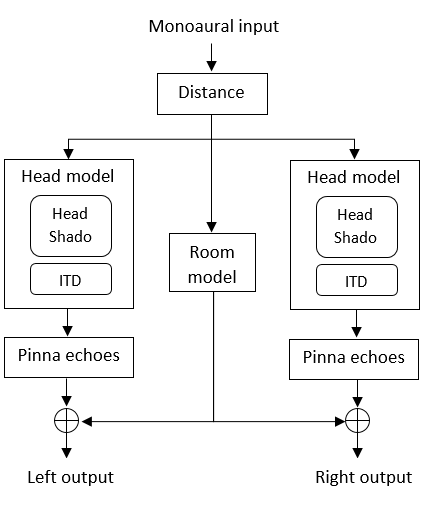
\includegraphics[scale=0.75]{graphics/graphic.png} 


We therefore used the analog filter models provided in \cite{Brown1997} and further specified in \cite{Brown1998}. The head shadow filter, implementing the ILD, was given by the following analog transfer function:
\begin{equation}\label{eq:analog}
H\left( s,\theta\right) = \frac{\alpha (\theta)s+\beta}{s+\beta},\: where\:\beta = \frac{2c}{a}
\end{equation}
Since this is an analog transfer function we had to derive the digital version by applying a bilinear transform applying the following substitution:
\begin{equation}\label{eq:bilin}
s = \frac{2}{T} \frac{z-1}{z+1},\: where\:T\:is\:???
\end{equation}
Applying the substitutin in Equation~\ref{eq:bilin} to Equation~\ref{eq:analog} we get the following filter function in the digital domain:
\begin{equation}\label{eq:filter}
H\left( z,\theta\right) = \frac{\alpha (\theta)(\frac{2}{T} \frac{z-1}{z+1})+\beta}{(\frac{2}{T} \frac{z-1}{z+1})+\beta}
\end{equation}
To identify the filter coefficients we transformed Equation ~\ref{eq:filter} and obtained the following frequency response\footnote{For the derivation of Equation~\ref{eq:filterparam} see appendix A}:
\begin{equation}\label{eq:filterparam}
H\left( z,\theta\right) = \frac{2\alpha (\theta)+T\beta+z^{-1}(-2\alpha(\theta)+T\beta)}{2+T\beta+z^{-1}(-2+T\beta)} = \frac{Y(z)}{X(z)}
\end{equation} 
This gives us the filter coefficients $a_0 = 2\alpha (\theta)+T\beta$ and $a_1 = -2\alpha(\theta)+T\beta$ as well as $b_0 = 2+T\beta$ and $b_1 = -2+T\beta$. Since we could not use the filter function in Matlab which has as input values the filter coefficientes we had to isolate the output $Y(z)$ in Equation~\ref{eq:filterparam} as well as going from the frequency to the time domain. The result is given in Equation~\ref{eq:out}\footnote{For the derivation of Equation~\ref{eq:out} see appendix B}:
\begin{equation}\label{eq:out}
Y[n] =\frac{a_0X[n]+a_1X[n-1]-b_1Y[n-1]}{b_0}
\end{equation} 

%%%%%%%%%%%%%%%%%%%%%%%%%%%%%%%%%%%%%%%%%%%%%%%%%%%%%%%%%%%%%%%%%%%%%%%%%%%%%%%%%%%%%%%%%%%%%%%%%%%%%
%%%%%%%%%%%%%%%%%%%%%%%%%%%%%%%%%%%%%%%%%%%%%%%%%%%%%%%%%%%%%%%%%%%%%%%%%%%%%%%%%%%%%%%%%%%%%%%%%%%%%


\subsection{User interface}
include pictures of user interface etc.

%%%%%%%%%%%%%%%%%%%%%%%%%%%%%%%%%%%%%%%%%%%%%%%%%%%%%%%%%%%%%%%%%%%%%%%%%%%%%%%%%%%%%%%%%%%%%%%%%%%%%
%%%%%%%%%%%%%%%%%%%%%%%%%%%%%%%%%%%%%%%%%%%%%%%%%%%%%%%%%%%%%%%%%%%%%%%%%%%%%%%%%%%%%%%%%%%%%%%%%%%%%
\section{Experimental design}

\subsection{Test group}

\subsection{Methodology and procedure}
As outlined in \cite{}, there is a lack of formal methodology on how to analyse and interpret user data that is not just qualitative, especially in an outdoor mobile audio-augmented reality environment. To supply it, we set out to design an initial pilot study by focusing on the user's performance and experience both qualitatively and quantitatively. 

(nr) users participate in the study. \textit{we could add something like this: they all reported normal hearing and were right-handed. (nr) of these users had used GPS-based systems before. None were paid for their participation. (nr) different participants tested each of the (n) auditory display conditions described in the previous section while (n) tested only conditions no. (set conditions). The experiment lasted no more than (set time)}.

First, user were asked to familiarize themselves with the system by [\ldots]. This procedure served to check the presence of the GPS signal inside the system prior to starting the test and also provide participants with the chance to ask question about the correct usage. They were then asked to [\ldots]. Participants were instructed to [\ldots]. At the end of each trial, participants were asked to fill a questionnaire and provide informal feedback about their experience. 

\subsection{Results}
We measured objective and subjective data on user performance. The objective measure we investigated were [\ldots], while for subjective analysis we present feedback from the participant questionnaire. 
\subsubsection{Quantitative analysis}
\subsubsection{User feedback}



\section{Discussion}
%%%%%%%%%%%%%%%%%%%%%%%%%%%%%%%%%%%%%%%%%%%%%%%%%%%%%%%%%%%%%%%%%%%%%%%%%%%%%%%%%%%%%%%%%%%%%%%%%%%%%
%%%%%%%%%%%%%%%%%%%%%%%%%%%%%%%%%%%%%%%%%%%%%%%%%%%%%%%%%%%%%%%%%%%%%%%%%%%%%%%%%%%%%%%%%%%%%%%%%%%%%


\section{Conclusion}


% conference papers do not normally have an appendix


% use section* for acknowledgment
\section*{Acknowledgment}


The authors would like to thank...Smilen and Stefania :)



\pagebreak
% Style and bibliography.
% The bibtex filename
\bibliography{}

% trigger a \newpage just before the given reference
% number - used to balance the columns on the last page
% adjust value as needed - may need to be readjusted if
% the document is modified later
%\IEEEtriggeratref{8}
% The "triggered" command can be changed if desired:
%\IEEEtriggercmd{\enlargethispage{-5in}}

% references section

% can use a bibliography generated by BibTeX as a .bbl file
% BibTeX documentation can be easily obtained at:
% http://mirror.ctan.org/biblio/bibtex/contrib/doc/
% The IEEEtran BibTeX style support page is at:
% http://www.michaelshell.org/tex/ieeetran/bibtex/
%\bibliographystyle{IEEEtran}
% argument is your BibTeX string definitions and bibliography database(s)
%\bibliography{IEEEabrv,../bib/paper}
%
% <OR> manually copy in the resultant .bbl file
% set second argument of \begin to the number of references
% (used to reserve space for the reference number labels box)
%\begin{thebibliography}{1}
%
%\bibitem{IEEEhowto:kopka}
%H.~Kopka and P.~W. Daly, \emph{A Guide to \LaTeX}, 3rd~ed.\hskip 1em plus
%  0.5em minus 0.4em\relax Harlow, England: Addison-Wesley, 1999.
%
%\end{thebibliography}

\pagebreak
\listoffigures
\pagebreak
\begin{appendices}
\section{Derivations}
\begin{equation*}\label{eq:DerivationFilterCoeff}
\begin{split}
H\left( z,\theta\right) &=\frac{\alpha (\theta)(\frac{2}{T} \frac{z-1}{z+1})+\beta}{(\frac{2}{T} \frac{z-1}{z+1})+\beta}\\
                                   &= \frac{\frac{2\alpha (\theta)(z-1)}{T(z+1)}+\frac{T\beta(z+1)}{T(z+1)}}{\frac{2(z-1)}{T(z+1)}+\frac{T\beta(z+1)}{T(z+1)}}\\  
			   &=\frac{\frac{2\alpha (\theta)(z-1)+T\beta(z+1)}{T(z+1)}}{\frac{2(z-1)+T\beta(z+1)}{T(z+1)}}\\
			  &=\frac{2\alpha (\theta)(z-1)+T\beta(z+1)}{2(z-1)+T\beta(z+1)}\\
			 &=\frac{z2\alpha (\theta)(1-z^{-1})+zT\beta(1+z^{-1})}{z2(1-z^{-1})+zT\beta(1+z^{-1})}\\
			&=\frac{2\alpha (\theta)(1-z^{-1})+T\beta(1+z^{-1})}{2(1-z^{-1})+T\beta(1+z^{-1})}\\
			&=\frac{2\alpha (\theta)-2\alpha (\theta)z^{-1}+T\beta+T\beta z^{-1}}{2-2z^{-1}+T\beta+T\beta z^{-1}}\\
			&=\frac{(2\alpha (\theta)+T\beta)-(2\alpha (\theta)+T\beta)z^{-1}}{(2+T\beta)-(2+T\beta)z^{-1}}\\
			&=\frac{(2\alpha (\theta)+T\beta)+(-2\alpha (\theta)+T\beta)z^{-1}}{(2+T\beta)+(-2+T\beta)z^{-1}}\\
\end{split}
\end{equation*} 
\section{Derivations}
\begin{equation*}\label{eq:DerivationC++}
\begin{split}
H(z, \theta) &= \frac{Y(z)}{X(z)} = \frac{a_0+a_1z^{-1}}{b_0+b_1z^{-1}}\\
&\iff Y(z)(b_0+b_1z^{-1}) = X(z)(a_0+a_1z^{-1})\\
&\iff Y(z)b_0+b_1Y(z)z^{-1} = a_0X(z)+a_1X(z)z^{-1}\\
&\iff Y(z) = \frac{a_0X(z)+a_1X(z)z^{-1}-b_1Y(z)z^{-1}}{b_0}\\
&\rightarrow Y[n] = \frac{a_0X[n]+a_1X[n-1]-b_1Y[n-1]}{b_0}
\end{split}
\end{equation*} 
\end{appendices}



% that's all folks
\end{document}


